%location/filename: tex/fig/ap7.tex
%author: Anders Østevik
%Last edited: 26.05.2016
%#######--Appendix - Soldering the ground pads--#######
%

\documentclass[main.tex]{subfiles}

\begin{document}

\chapter{Soldering the Ground Pads Underneath the HSMC Contact} \label{ap:solder}

The \gls{hsmc}-connector has several ground pads underneath the connector itself, making it impossible to reach when soldering by hand. The solution was to use a solder oven with solder paste on the pads. The solder paste was applied on the pads with the help of the dispenser module on the \textit{Martin Rework Station}, which was available in the lab. The dispenser module forces the solder paste out of the syringe using pressurized air. By pressing a foot pedal connected to the dispenser, you apply a controlled air pulse that pushes on the piston of the solder paste syringe. The force of the air pulse can be adjusted using the dispenser \acrshort{gui}. For the ground pads, an air flow of $2.50~CMM$ (Cubic Meter per Minute) was suitable.

The solder oven that was used had the option to set up a \textit{Ramp-Soak-Spike} type thermal profile. Samtec, the manufacturer for the \gls{hsmc} contact, recommends a maximum peak temperature of no more than $260~\degree C$ with no more than 30 seconds above $255\degree C$. The thermal profile setup is based on the profile recommended by EFD, the manufacturer for the particular solder paste used (see figure \ref{fig:krepro}). After some trial and error with a dummy-PCB, the oven was set to a activation temperature of $150\degree C$ for $60~seconds$, and then a reflow temperature of $220\degree C$ with a climb-time of $120~seconds$. 

\begin{figure}[H] % H(strictly put HERE > h!)
% h(here), !(force), t(top), b(bottom), p(on extra page)
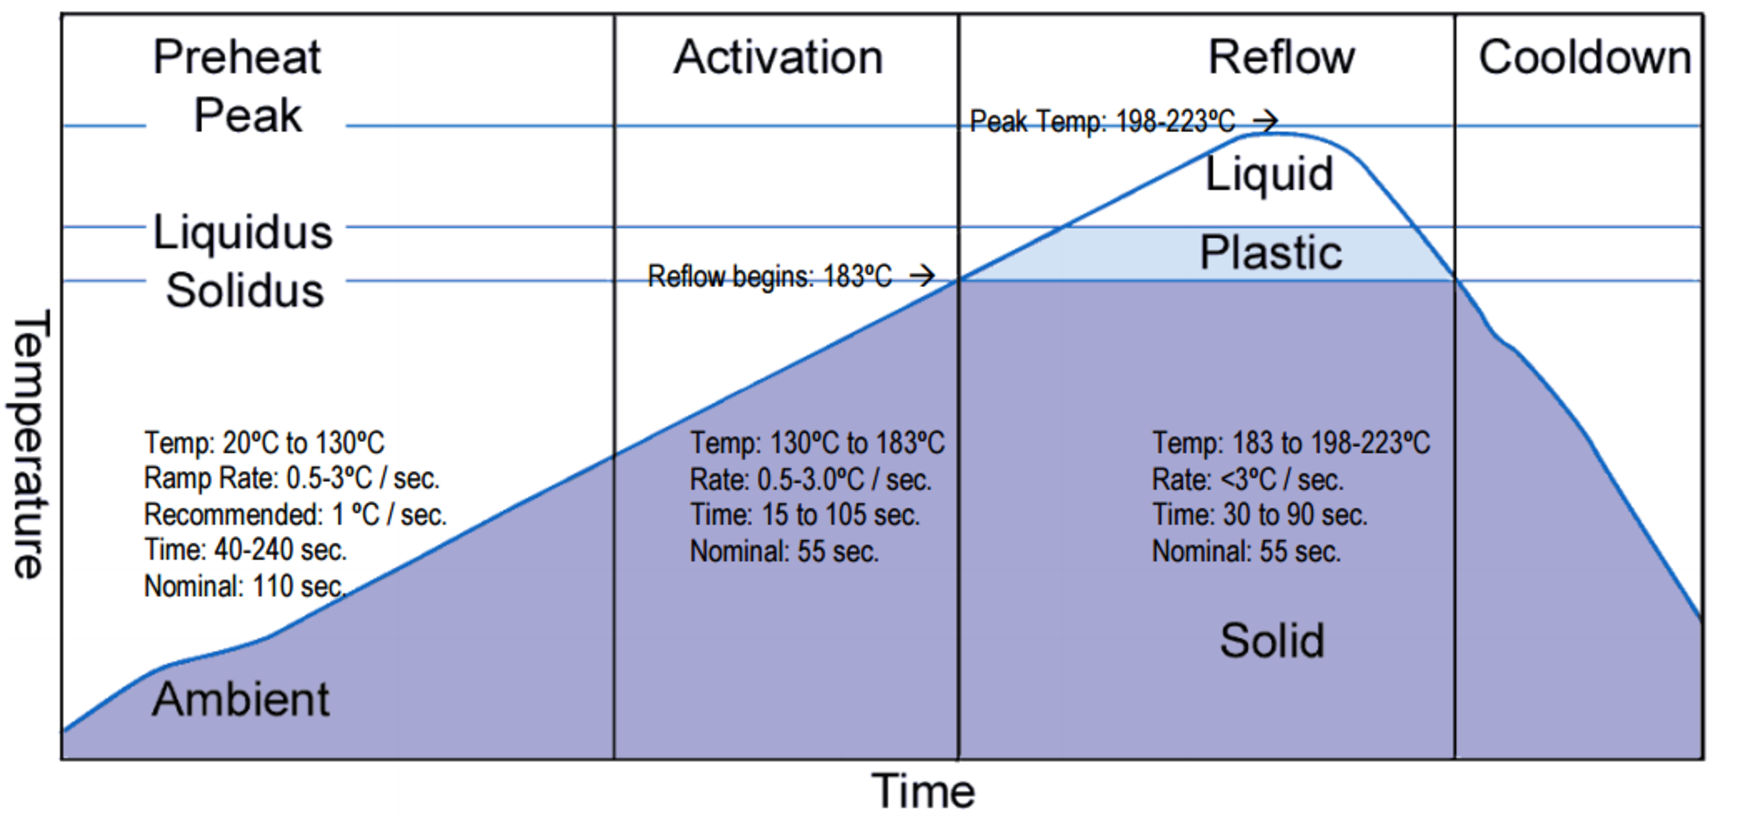
\includegraphics[width=0.8\linewidth]{../img/temp_prof}  \\[0.1 cm]
\caption{EFD reflow thermal profile recommendations \cite{krepro_reflow}.}
\label{fig:krepro}
\end{figure}

\end{document}


